\documentclass[a4paper,twoside,10pt]{dynadoc}

% enlarge the page a bit..
% \addtolength{\hoffset}{-1cm}
% \addtolength{\textwidth}{2cm}
% \addtolength{\voffset}{-1.5cm}
% \addtolength{\textheight}{3cm}

\usepackage{latexsym}
\usepackage{amssymb}
%\usepackage{tabularx}
\usepackage{ltxtable}
\usepackage{hyperref}
\usepackage{wrapfig}

\title{DHTML Calendar Widget}
\author{Mihai Bazon, \texttt{<mihai\_bazon@yahoo.com>}\\
\copyright\ Dynarch.com 2002--2005, \href{http://www.dynarch.com/}{\texttt{www.dynarch.com}}}
\date{\today\\\vspace{0.2ex}
{\small calendar version: 1.0 ``It is happening again''}
}

\begin{document}

\maketitle

{\small\verb|$Id: reference.tex,v 1.23 2005/03/05 11:37:14 mishoo Exp $|}
{\begin{small}\begin{quote}
{\begin{flushright}
\noindent
\end{flushright}}
\end{quote}\end{small}}
\tableofcontents

% \setlength{\parindent}{0pt}
% \setlength{\parskip}{1.3ex}

\section{Overview}

The DHTML Calendar widget\footnote
        {
        by the term ``widget'' I understand a single element of user interface.
        But that's in Linux world.  For those that did lots of Windows
        programming the term ``control'' might be more familiar
        }
is an (HTML) user interface element that gives end-users a friendly way to
select date and time.  It works in a web browser.  The first versions only provided
support for popup calendars, while starting with version 0.9 it also supports
``flat'' display.  A ``flat'' calendar is a calendar that stays visible in the
page all the time.  In this mode it could be very useful for ``blog'' pages and
other pages that require the calendar to be always present.

The calendar is compatible with most popular browsers nowadays.  While it's
created using web standards and it should generally work with any compliant
browser, the following browsers were found to work: Mozilla/Firefox (the
development platform), Netscape~6.0 or better, all other Gecko-based browsers,
Internet Explorer~5.0 or better \emph{for Windows}\footnote{people report that the calendar does
not work with IE5/Mac.  However, this browser was discontinued and we
believe that supporting it doesn't worth the efforts, given the fact that
it has the worst, buggiest implementation for DOM I've ever seen.}, Opera~7\footnote
        { under Opera 7 the calendar still lacks some functionality, such as
        keyboard navigation; also Opera doesn't seem to allow disabling text
        selection when one drags the mouse on the page; despite all that, the
        calendar is still highly functional under Opera 7 and looks as good as
        in other supported browsers. }, Konqueror 3.1.2 and Apple Safari for
MacOSX.

You can find the latest info and version at the calendar homepage:

\begin{center}
{\href{http://www.dynarch.com/projects/calendar/}
{\texttt{www.dynarch.com/projects/calendar}}}
\end{center}

\subsection{How does this thing work?}

DHTML is not ``another kind of HTML''.  It's merely a naming convention.  DHTML
refers to the combination of HTML, CSS, JavaScript and DOM.  DOM (Document
Object Model) is a set of interfaces that glues the other three together.  In
other words, DOM allows dynamic modification of an HTML page through a program.
JavaScript is our programming language, since that's what browsers like.  CSS
is a way to make it look good ;-).  So all this soup is generically known as
DHTML.

Using DOM calls, the program dynamically creates a \texttt{<table>} element
that contains a calendar for the given date and then inserts it in the document
body.  Then it shows this table at a specified position.  Usually the position
is related to some element in which the date needs to be displayed/entered,
such as an input field.

By assigning a certain CSS class to the table we can control the look of the
calendar through an external CSS file; therefore, in order to change the
colors, backgrounds, rollover effects and other stuff, you can only change a
CSS file---modification of the program itself is not necessary.

\subsection{Project files}

Here's a description of the project files, excluding documentation and example
files.

\begin{itemize}

\item the main program file (\texttt{calendar.js}).  This defines all the logic
behind the calendar widget.

\item the CSS files (\texttt{calendar-*.css}).  Loading one of them is
necessary in order to see the calendar as intended.

\item the language definition files (\texttt{lang/calendar-*.js}).  They are
plain JavaScript files that contain all texts that are displayed by the
calendar.  Loading one of them is necessary.

\item helper functions for quick setup of the calendar
(\texttt{calendar-setup.js}).  You can do fine without it, but starting with
version 0.9.3 this is the recommended way to setup a calendar.

\end{itemize}

\subsection{License}

\begin{center}
\noindent \copyright\ Dynarch.com 2002--2005,
\href{http://www.dynarch.com/}{\texttt{www.dynarch.com}}\\
Author: Mihai Bazon
\end{center}

The calendar is released under the
{\href{http://www.gnu.org/licenses/lgpl.html}{GNU Lesser General Public License}}.




\section{Quick startup}\label{sec:quick-start}

Installing the calendar used to be quite a task until version 0.9.3.  Starting
with 0.9.3 I have included the file \texttt{calendar-setup.js} whose goal is to
assist you to setup a popup or flat calendar in minutes.  You are
encouraged to modify this file and \emph{not} calendar.js if you need
extra customization, but you're on your own.

First you have to include the needed scripts and style-sheet.  Make sure you do
this in your document's \texttt{<head>} section, also make sure you put the
correct paths to the scripts.

\begin{verbatim}
<style type="text/css">@import url(calendar-win2k-1.css);</style>
<script type="text/javascript" src="calendar.js"></script>
<script type="text/javascript" src="lang/calendar-en.js"></script>
<script type="text/javascript" src="calendar-setup.js"></script>
\end{verbatim}

\subsection{Installing a popup calendar}\label{sec:quick-start-popup}

\noindent Now suppose you have the following HTML:

\begin{verbatim}
<form ...>
  <input type="text" id="data" name="data" />
  <button id="trigger">...</button>
</form>
\end{verbatim}

\noindent You want the button to popup a calendar widget when clicked?  Just
insert the following code immediately \emph{after} the HTML form:

\begin{verbatim}
<script type="text/javascript">
  Calendar.setup(
    {
      inputField  : "data",         // ID of the input field
      ifFormat    : "%m %d, %Y",    // the date format
      button      : "trigger"       // ID of the button
    }
  );
</script>
\end{verbatim}

The \texttt{Calendar.setup} function, defined in \texttt{calendar-setup.js}
takes care of ``patching'' the button to display a calendar when clicked.  The
calendar is by default in single-click mode and linked with the given input
field, so that when the end-user selects a date it will update the input field
with the date in the given format and close the calendar.  If you are a
long-term user of the calendar you probably remember that for doing this you
needed to write a couple functions and add an ``onclick'' handler for the
button by hand.

By looking at the example above we can see that the function
\texttt{Calendar.setup} receives only one parameter: a JavaScript object.
Further, that object can have lots of properties that tell to the setup
function how would we like to have the calendar.  For instance, if we would
like a calendar that closes at double-click instead of single-click we would
also include the following: \texttt{singleClick:false}.

For a list of all supported parameters please see the section
\ref{sec:Calendar.setup}.

\subsection{Installing a flat calendar}\label{sec:quick-start-flat}

Here's how to configure a flat calendar, using the same \texttt{Calendar.setup}
function.  First, you should have an empty element with an ID.  This element
will act as a container for the calendar.  It can be any block-level element,
such as DIV, TABLE, etc.  We will use a DIV in this example.

\begin{verbatim}
<div id="calendar-container"></div>
\end{verbatim}

Then there is the JavaScript code that sets up the calendar into the
``calendar-container'' DIV.  The code can occur anywhere in HTML
\emph{after} the DIV element.

\begin{verbatim}
<script type="text/javascript">
  function dateChanged(calendar) {
    // Beware that this function is called even if the end-user only
    // changed the month/year.  In order to determine if a date was
    // clicked you can use the dateClicked property of the calendar:
    if (calendar.dateClicked) {
      // OK, a date was clicked, redirect to /yyyy/mm/dd/index.php
      var y = calendar.date.getFullYear();
      var m = calendar.date.getMonth();     // integer, 0..11
      var d = calendar.date.getDate();      // integer, 1..31
      // redirect...
      window.location = "/" + y + "/" + m + "/" + d + "/index.php";
    }
  };

  Calendar.setup(
    {
      flat         : "calendar-container", // ID of the parent element
      flatCallback : dateChanged           // our callback function
    }
  );
</script>
\end{verbatim}

\subsection{\texttt{Calendar.setup} in detail}\label{sec:Calendar.setup}

Following there is the complete list of properties interpreted by
Calendar.setup.  All of them have default values, so you can pass only those
which you would like to customize.  Anyway, you \emph{must} pass at least one
of \texttt{inputField}, \texttt{displayArea} or \texttt{button}, for a popup
calendar, or \texttt{flat} for a flat calendar.  Otherwise you will get a
warning message saying that there's nothing to setup.

\begin{small}
\ifx\shipout\undefined
\begin{tabular}{l l l r}
\textbf{property} & \textbf{type} & \textbf{description} & \textbf{default}
\\\hline\hline
\endhead
\texttt{inputField}
& string & The ID of your input field.
& null
\\\hline
\texttt{displayArea}
& string & This is the ID of a $<$span$>$, $<$div$>$, or any other element that you would like to use to display the current date. This is generally useful only if the input field is hidden, as an area to display the date.
& null
\\\hline
\texttt{button}
& string & The ID of the calendar ``trigger''. This is an element (ordinarily a button or an image) that will dispatch a certain event (usually ``click'') to the function that creates and displays the calendar.
& null
\\\hline
\texttt{eventName}
& string & The name of the event that will trigger the calendar. The name should be without the ``on'' prefix, such as ``click'' instead of ``onclick''. Virtually all users will want to let this have the default value (``click''). Anyway, it could be useful if, say, you want the calendar to appear when the input field is focused and have no trigger button (in this case use ``focus'' as the event name).
& ``click''
\\\hline
\texttt{ifFormat}
& string & The format string that will be used to enter the date in the input field. This format will be honored even if the input field is hidden.
& ``\%Y/\%m/\%d''
\\\hline
\texttt{daFormat}
& string & Format of the date displayed in the displayArea (if specified).
& ``\%Y/\%m/\%d''
\\\hline
\texttt{singleClick}
& boolean & Wether the calendar is in ``single-click mode'' or ``double-click mode''. If true (the default) the calendar will be created in single-click mode.
& true
\\\hline
\texttt{disableFunc}
& function & A function that receives a JS Date object.  It should return
\texttt{true} if that date has to be disabled, \texttt{false} otherwise.
{\color{red} DEPRECATED (see below).}
& null
\\\hline
\texttt{dateStatusFunc}
& function & A function that receives a JS Date object and returns a boolean
or a string.  This function allows one to set a certain CSS class to some
date, therefore making it look different.  If it returns \texttt{true} then
the date will be disabled.  If it returns \texttt{false} nothing special
happens with the given date.  If it returns a string then that will be taken
as a CSS class and appended to the date element.  If this string is
``disabled'' then the date is also disabled (therefore is like returning
\texttt{true}).  For more information please also refer to section
\ref{sec:Calendar.setDateStatusHandler}.
& null
\\\hline
\texttt{firstDay}
& integer & Specifies which day is to be displayed as the first day of
week.  Possible values are 0 to 6; 0 means Sunday, 1 means Monday, ..., 6
means Saturday.  The end user can easily change this too, by clicking on the
day name in the calendar header.
& 0
\\\hline
\texttt{weekNumbers}
& boolean & If ``true'' then the calendar will display week numbers.
& true
\\\hline
\texttt{align}
& string & Alignment of the calendar, relative to the reference element. The
reference element is dynamically chosen like this: if a displayArea is
specified then it will be the reference element. Otherwise, the input field
is the reference element.  For the meaning of the alignment characters
please section \ref{sec:Calendar.showAtElement}.
& ``Bl''
\\\hline
\texttt{range}
& array & An array having exactly 2 elements, integers. (!) The first [0] element is the minimum year that is available, and the second [1] element is the maximum year that the calendar will allow.
& [1900, 2999]
\\\hline
\texttt{flat}
& string & If you want a flat calendar, pass the ID of the parent object in
this property.  If not, pass \texttt{null} here (or nothing at all as
\texttt{null} is the default value).
& null
\\\hline
\texttt{flatCallback}
& function & You should provide this function if the calendar is flat.  It
will be called when the date in the calendar is changed with a reference to
the calendar object.  See section \ref{sec:quick-start-flat} for an example
of how to setup a flat calendar.
& null
\\\hline
\texttt{onSelect}
& function & If you provide a function handler here then you have to manage
the ``click-on-date'' event by yourself.  Look in the calendar-setup.js and
take as an example the onSelect handler that you can see there.
& null
\\\hline
\texttt{onClose}
& function & This handler will be called when the calendar needs to close.
You don't need to provide one, but if you do it's your responsibility to
hide/destroy the calendar.  You're on your own.  Check the calendar-setup.js
file for an example.
& null
\\\hline
\texttt{onUpdate}
& function & If you supply a function handler here, it will be called right
after the target field is updated with a new date.  You can use this to
chain 2 calendars, for instance to setup a default date in the second just
after a date was selected in the first.
& null
\\\hline
\texttt{date}
& date & This allows you to setup an initial date where the calendar will be
positioned to.  If absent then the calendar will open to the today date.
& null
\\\hline
\texttt{showsTime}
& boolean & If this is set to \texttt{true} then the calendar will also
allow time selection.
& false
\\\hline
\texttt{timeFormat}
& string & Set this to ``12'' or ``24'' to configure the way that the
calendar will display time.
& ``24''
\\\hline
\texttt{electric}
& boolean & Set this to ``false'' if you want the calendar to update the
field only when closed (by default it updates the field at each date change,
even if the calendar is not closed) & true
\\\hline
\texttt{position}
& array & Specifies the [x, y] position, relative to page's top-left corner,
where the calendar will be displayed.  If not passed then the position will
be computed based on the ``align'' parameter.  Defaults to ``null'' (not
used). & null
\\\hline
\texttt{cache}
& boolean & Set this to ``true'' if you want to cache the calendar object.
This means that a single calendar object will be used for all fields that
require a popup calendar & false
\\\hline
\texttt{showOthers}
& boolean & If set to ``true'' then days belonging to months overlapping
with the currently displayed month will also be displayed in the calendar
(but in a ``faded-out'' color) & false

\end{tabular}

\else
\LTXtable{\textwidth}{Calendar.setup.pdf.tex}
\fi
\end{small}




\section{Recipes}

This section presents some common ways to setup a calendar using the
\texttt{Calendar.setup} function detailed in the previous section.

We don't discuss here about loading the JS or CSS code---so make sure you
add the proper $<$script$>$ and $<$style$>$ or $<$link$>$ elements in your
HTML code.  Also, when we present input fields, please note that they should
be embedded in some form in order for data to be actually sent to server; we
don't discuss these things here because they are not related to our
calendar.

\subsection{Popup calendars}

These samples can be found in the file “\texttt{simple-1.html}” from the
calendar package.

\subsubsection{Simple text field with calendar attached to a button}

% \begin{wrapfigure}{r}{5cm}
% 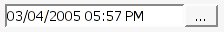
\includegraphics{field-button}
% \end{wrapfigure}

This piece of code will create a calendar for a simple input field with a
button that will open the calendar when clicked.

\begin{verbatim}
<input type="text" name="date" id="f_date_b"
       /><button type="reset" id="f_trigger_b"
       >...</button>
<script type="text/javascript">
    Calendar.setup({
        inputField     :    "f_date_b",           //*
        ifFormat       :    "%m/%d/%Y %I:%M %p",
        showsTime      :    true,
        button         :    "f_trigger_b",        //*
        step           :    1
    });
</script>
\end{verbatim}

Note that this code does more actually; the only \emph{required} fields are
those marked with “//$*$”---that is, the ID of the input field and the ID of
the button need to be passed to \texttt{Calendar.setup} in order for the
calendar to be properly assigned to this input field.  As one can easily
guess from the argument names, the other arguments configure a certain date
format, instruct the calendar to also include a time selector and display
every year in the drop-down boxes (the “step” parameter)---instead of showing
every other year as the default calendar does.

\subsubsection{Simple field with calendar attached to an image}

Same as the above, but the element that triggers the calendar is this time
an image, not a button.

\begin{verbatim}
<input type="text" name="date" id="f_date_c" readonly="1" />
<img src="img.gif" id="f_trigger_c"
     style="cursor: pointer; border: 1px solid red;"
     title="Date selector"
     onmouseover="this.style.background='red';"
     onmouseout="this.style.background=''" />
<script type="text/javascript">
    Calendar.setup({
        inputField     :    "f_date_c",
        ifFormat       :    "%B %e, %Y",
        button         :    "f_trigger_c",
        align          :    "Tl",
        singleClick    :    false
    });
</script>
\end{verbatim}

Note that the same 2 parameters are required as in the previous case; the
difference is that the 'button' parameter now gets the ID of the image
instead of the ID of the button.  But the event is the same: at 'onclick' on
the element that is passed as 'button', the calendar will be shown.

The above code additionally sets an alignment mode---the parameters are
described in \ref{sec:Calendar.showAtElement}.

\subsubsection{Hidden field, plain text triggers}

Sometimes, to assure that the date is well formatted, you might want not to
allow the end user to write a date manually.  This can easily be achieved
with an input field by setting its \texttt{readonly} attribute, which is
defined by the HTML4 standard; however, here's an even nicer approach: our
calendar widget allows you to use a hidden field as the way to pass data to
server, and a “display area” to show the end user the selected date.  The
“display area” can be any HTML element, such as a DIV or a SPAN or
whatever---we will use a SPAN in our sample.

\begin{verbatim}
<input type="hidden" name="date" id="f_date_d" />

<p>Your birthday:
   <span style="background-color: #ff8; cursor: default;"
         onmouseover="this.style.backgroundColor='#ff0';"
         onmouseout="this.style.backgroundColor='#ff8';"
         id="show_d"
   >Click to open date selector</span>.</p>

<script type="text/javascript">
    Calendar.setup({
        inputField     :    "f_date_d",
        ifFormat       :    "%Y/%d/%m",
        displayArea    :    "show_d",
        daFormat       :    "%A, %B %d, %Y",
    });
</script>
\end{verbatim}

The above code will configure a calendar attached to the hidden field and to
the SPAN having the id=“show\_d”.  When the SPAN element is clicked, the
calendar opens and allows the end user to chose a date.  When the date is
chosen, the input field will be updated with the value in the format
“\texttt{\%Y/\%d/\%m}”, and the SPAN element will display the date in a
friendlier format (defined by “\texttt{daFormat}”).

Beware that using this approach will make your page unfunctional in browsers
that do not support JavaScript or our calendar.

\subsubsection{2 Linked fields, no trigger buttons}

Supposing you want to create 2 fields that hold an interval of exactly one
week.  The first is the starting date, and the second is the ending date.
You want the fields to be automatically updated when some date is clicked in
one or the other, in order to keep exactly one week difference between them.

\begin{verbatim}
<input type="text" name="date" id="f_date_a" />
<input type="text" name="date" id="f_calcdate" />

<script type="text/javascript">
    function catcalc(cal) {
        var date = cal.date;
        var time = date.getTime()
        // use the _other_ field
        var field = document.getElementById("f_calcdate");
        if (field == cal.params.inputField) {
            field = document.getElementById("f_date_a");
            time -= Date.WEEK; // substract one week
        } else {
            time += Date.WEEK; // add one week
        }
        var date2 = new Date(time);
        field.value = date2.print("%Y-%m-%d %H:%M");
    }
    Calendar.setup({
        inputField     :    "f_date_a",
        ifFormat       :    "%Y-%m-%d %H:%M",
        showsTime      :    true,
        timeFormat     :    "24",
        onUpdate       :    catcalc
    });
    Calendar.setup({
        inputField     :    "f_calcdate",
        ifFormat       :    "%Y-%m-%d %H:%M",
        showsTime      :    true,
        timeFormat     :    "24",
        onUpdate       :    catcalc
    });
</script>
\end{verbatim}

The above code will configure 2 input fields with calendars attached, as
usual.  The first thing to note is that there's no trigger button---in such
case, the calendar will popup when one clicks into the input field.  Using
the \texttt{onUpdate} parameter, we pass a reference to a function of ours
that will get called after a date was selected.  In that function we
determine what field was updated and we compute the date in the other input
field such that it keeps a one week difference between the two.  Enjoy! :-)

\subsection{Flat calendars}

This sample can be found in “\texttt{simple-2.html}”.  It will configure a
flat calendar that is always displayed in the page, in the DIV having the
id=“calendar-container”.  When a date is clicked our function hander gets
called (\texttt{dateChanged}) and it will compute an URL to jump to based on
the selected date, then use \texttt{window.location} to visit the new link.

\begin{verbatim}
<div style="float: right; margin-left: 1em; margin-bottom: 1em;"
id="calendar-container"></div>

<script type="text/javascript">
  function dateChanged(calendar) {
    // Beware that this function is called even if the end-user only
    // changed the month/year.  In order to determine if a date was
    // clicked you can use the dateClicked property of the calendar:
    if (calendar.dateClicked) {
      // OK, a date was clicked, redirect to /yyyy/mm/dd/index.php
      var y = calendar.date.getFullYear();
      var m = calendar.date.getMonth();     // integer, 0..11
      var d = calendar.date.getDate();      // integer, 1..31
      // redirect...
      window.location = "/" + y + "/" + m + "/" + d + "/index.php";
    }
  };

  Calendar.setup(
    {
      flat         : "calendar-container", // ID of the parent element
      flatCallback : dateChanged           // our callback function
    }
  );
</script>
\end{verbatim}

\subsection{Highlight special dates}

So you want to display certain dates in a different color, or with bold
font, or whatever, right?  Well, no problem---our calendar can do this as
well.  It doesn't matter if it's a flat or popup calendar---we'll use a flat
one for this sample.  The idea, however, is that you need to have the dates
in an array or a JavaScript object---whatever is suitable for your way of
thinking---and use it from a function that returns a value, telling the
calendar what kind of date is the passed one.

Too much talking, here's the code ;-)

\begin{verbatim}
<!-- this goes into the <head> tag -->
<style type="text/css">
  .special { background-color: #000; color: #fff; }
</style>

<!-- and the rest inside the <body> -->
<div style="float: right; margin-left: 1em; margin-bottom: 1em;"
id="calendar-container"></div>

<script type="text/javascript">
  var SPECIAL_DAYS = {
    0 : [ 13, 24 ],		// special days in January
    2 : [ 1, 6, 8, 12, 18 ],	// special days in March
    8 : [ 21, 11 ]		// special days in September
  };

  function dateIsSpecial(year, month, day) {
    var m = SPECIAL_DAYS[month];
    if (!m) return false;
    for (var i in m) if (m[i] == day) return true;
    return false;
  };

  function dateChanged(calendar) {
    // Beware that this function is called even if the end-user only
    // changed the month/year.  In order to determine if a date was
    // clicked you can use the dateClicked property of the calendar:
    if (calendar.dateClicked) {
      // OK, a date was clicked, redirect to /yyyy/mm/dd/index.php
      var y = calendar.date.getFullYear();
      var m = calendar.date.getMonth();     // integer, 0..11
      var d = calendar.date.getDate();      // integer, 1..31
      // redirect...
      window.location = "/" + y + "/" + m + "/" + d + "/index.php";
    }
  };

  function ourDateStatusFunc(date, y, m, d) {
    if (dateIsSpecial(y, m, d))
      return "special";
    else
      return false; // other dates are enabled
      // return true if you want to disable other dates
  };

  Calendar.setup(
    {
      flat         : "calendar-container", // ID of the parent element
      flatCallback : dateChanged,          // our callback function
      dateStatusFunc : ourDateStatusFunc
    }
  );
</script>
\end{verbatim}

So the above code creates a normal flat calendar, like in the previous
sample.  We hook into it with the function “\texttt{ourDateStatusFunc}”,
which receives a date object as the first argument, and also the year,
month, date as the next 3 arguments (normally, you can extract year, month,
date from the first parameter too, but we pass them separately for
convenience, as it's very likely that they are going to be used in this
function).

So, this function receives a date.  It can return \texttt{false} if you want
no special action to be taken on that date, \texttt{true} if that date
should be disabled (unselectable), or a string if you want to assign a
special CSS class to that date.  We return “special” for the dates that we
want to highlight---and note that we defined a “special” look for them in
the CSS section.

I used a simple approach here to define what dates are special.  There's a
JavaScript object (the SPECIAL\_DAYS global variable) which holds an array
of dates for each month.  Month numbers start at zero (January).  Months
that don't contain special dates can be absent from this object.  Note that
the way to implement this is completely separated from the calendar
code---therefore, feel free to use your imagination if you have better
ideas. :-)

\subsection{Select multiple dates}

Starting version 1.0, the calendar is able to handle multiple dates
selection.  You just need to pass the “\texttt{multiple}” parameter to
\texttt{Calendar.setup} and add some special code that interprets the
selection once the calendar is closed.

\begin{verbatim}
<a id="trigger" href="#">[open calendar...]</a>
<div id="output"></div>
<script type="text/javascript">//<![CDATA[
    // the default multiple dates selected,
    // first time the calendar is displayed
    var MA = [];

    function closed(cal) {

      // here we'll write the output; this is only for example.  You
      // will normally fill an input field or something with the dates.
      var el = document.getElementById("output");

      // reset initial content.
      el.innerHTML = "";

      // Reset the "MA", in case one triggers the calendar again.
      // CAREFUL!  You don't want to do "MA = [];".  We need to modify
      // the value of the current array, instead of creating a new one.
      // Calendar.setup is called only once! :-)  So be careful.
      MA.length = 0;

      // walk the calendar's multiple dates selection hash
      for (var i in cal.multiple) {
        var d = cal.multiple[i];
        // sometimes the date is not actually selected,
        // so let's check
        if (d) {
          // OK, selected.  Fill an input field or something.
          el.innerHTML += d.print("%A, %Y %B %d") + "<br />";
          // and push it in the "MA", in case one triggers the calendar again.
          MA[MA.length] = d;
        }
      }
      cal.hide();
      return true;
    };

    Calendar.setup({
      align      : "BR",
      showOthers : true,
      multiple   : MA, // pass the initial or computed array of multiple dates
      onClose    : closed,
      button     : "trigger"
    });
//]]></script>
\end{verbatim}

The above code creates a popup calendar and passes to it an array of dates,
which is initially empty, in the “multiple” argument.  When the calendar is
closed it will call our “\texttt{closed}” function handler; in this handler
we determine what dates were actually selected, inspecting the
“\texttt{cal.multiple}” property, we display them in a DIV element right
next to the $<$a$>$ element that opens the calendar, and we reinitialize the
global array of selected dates (which will be used if the end user opens the
calendar again).  I guess the code speaks for itself, right? :-)




\section{The Calendar object overview}\label{sec:Calendar_overview}

Basically you should be able to setup the calendar with the function presented
in the previous section.  However, if for some reason \texttt{Calendar.setup}
doesn't provide all the functionality that you need and you want to tweak into
the process of creating and configuring the calendar ``by hand'', then this
section is the way to go.

The file \texttt{calendar.js} implements the functionality of the calendar.
All (well, almost all) functions and variables are embedded in the JavaScript
object ``Calendar''.

You can instantiate a \texttt{Calendar} object by calling the constructor, like
this: \texttt{var cal = new Calendar(\ldots)}.  We will discuss the parameters
later.  After creating the object, the variable \texttt{cal} will contain a
reference to it.  You can use this reference to access further options of the
calendar, for instance:

\begin{verbatim}
cal.weekNumbers = false; // do not display week numbers
cal.showsTime = true;    // include a time selector
cal.setDateFormat("%Y.%m.%d %H:%M"); // set this format: 2003.12.31 23:59
cal.setDisabledHandler(function(date, year, month, day) {
  // verify date and return true if it has to be disabled
  // ``date'' is a JS Date object, but if you only need the
  // year, month and/or day you can get them separately as
  // next 3 parameters, as you can see in the declaration
  if (year == 2004) {
    // disable all dates from 2004
    return true;
  }
  return false;
});
\end{verbatim}

\noindent etc.  Prior to version
0.9.3 this was the only way to configure it.  The \texttt{Calendar.setup}
function, documented in section \ref{sec:quick-start}, basically does the same
things (actually more) in order to setup the calendar, based on the parameters
that you provided.

\subsection{Creating a calendar}

The calendar is created by following some steps (even the function
\texttt{Calendar.setup}, described in section \ref{sec:quick-start}, does the
same).  While you can skip optional (marked ``opt'') steps if you're happy with
the defaults, please respect the order below.

\begin{enumerate}

\item \emph{Instantiate} a \texttt{Calendar} object.  Details about this in
section \ref{sec:Calendar.constructor}.

\item [opt] Set the \texttt{weekNumbers} property to \texttt{false} if you don't want
the calendar to display week numbers.

\item [opt] Set the \texttt{showsTime} property to \texttt{true} if you
want the calendar to also provide a time selector.

\item [opt] Set the \texttt{time24} property to \texttt{false} if you want
the time selector to be in 12-hour format.  Default is 24-hour format.  This
property only has effect if you also set \texttt{showsTime} to
\texttt{true}.

\item [opt] Set the range of years available for selection (see section
\ref{sec:Calendar.setRange}).  The default range is [1970..2050].

\item [opt] Set the \texttt{getDateStatus} property.  You should pass
here a function that receives a JavaScript \texttt{Date} object and returns
\texttt{true} if the given date should be disabled, false otherwise (details in
section \ref{sec:Calendar.setDisabledHandler}).

\item [opt] Set a date format.  Your handler function, passed to the
calendar constructor, will be called when a date is selected with a reference
to the calendar and a date string in this format.

\item \emph{Create} the HTML elements related to the calendar.  This step
practically puts the calendar in your HTML page.  You simply call
\texttt{Calendar.create()}.  You can give an optional parameter if you wanna
create a flat calendar (details in section \ref{sec:Calendar.create}).

\item [opt] Initialize the calendar to a certain date, for instance from
the input field.

\item Show the calendar (details in section \ref{sec:Calendar.show}).

\end{enumerate}

\subsection{Order does matter ;-)}

As you could see in the previous section, there are more steps to be followed
in order to setup the calendar.  This happens because there are two different
things that need to be accomplished: first there is the JavaScript object, that
is created with \texttt{new Calendar(\ldots)}.  Secondly there are the HTML
elements that actually lets you see and manipulate the calendar.

{\begin{small}
[ Those that did UI\footnote{user interface} programming, no matter in what
language and on what platform, may be familiar with this concept.  First there
is the object in memory that lets you manipulate the UI element, and secondly
there is the UI element (known as ``control'', ``window'', ``widget'', etc.),
also in memory but you don't usually access it directly. ]
\end{small}}

By instantiating the calendar we create the JavaScript object.  It lets us
configure some properties and it also knows how to create the UI element (the
HTML elements actually) that will eventually be what the end-user sees on
screen.  Creation of the HTML element is accomplished by the function
\texttt{Calendar.create}.  It knows how to create popup or flat calendars.
This function is described in section \ref{sec:Calendar.create}.

Some properties need to be set prior to creating the HTML elements, because
otherwise they wouldn't have any effect.  Such a property is
\texttt{weekNumbers}---it has the default value ``true'', and if you don't
want the calendar to display the week numbers you have to set it to false.  If,
however, you do that \emph{after} calling \texttt{Calendar.create} the calendar
would still display the week numbers, because the HTML elements are already
created (including the \texttt{<td>}-s in the \texttt{<table>} element that
should contain the week numbers).  For this reason the order of the steps above
is important.

Another example is when you want to show the calendar.  The ``create'' function
does create the HTML elements, but they are initially hidden (have the style
``display: none'') unless the calendar is a flat calendar that should be always
visible in the page.  Obviously, the \texttt{Calendar.show} function should be
called \emph{after} calling \texttt{Calendar.create}.

\subsection{Caching the object}

Suppose the end-user has popped up a calendar and selects a date.  The calendar
then closes.  What really happens now?

There are two approaches.  The first (used in very old versions of the
calendar) was to drop completely the Calendar object and when the end-user pops
up the calendar again to create another one.  This approach is bad for more
reasons:

\begin{itemize}

\item creating the JavaScript object and HTML elements is time-consuming

\item we may loose some end-user preferences (i.e. he might prefer to have
Monday for the first day of week and probably already clicked it the first time
when the calendar was opened, but now he has to do it again)

\end{itemize}

The second approach, implemented by the \texttt{Calendar.setup} function, is to
cache the JavaScript object.  It does this by checking the global variable
\texttt{window.calendar} and if it is not null it assumes it is the created
Calendar object.  When the end-user closes the calendar, our code will only
call ``\texttt{hide}'' on it, therefore keeping the JavaScript object and the
HTML elements in place.

{\color{red} CAVEAT:} \quad Since time selection support was introduced, this
``object caching'' mechanism has the following drawback: if you once created
the calendar with the time selection support, then other items that may not
require this functionality will still get a calendar with the time selection
support enabled.  And reciprocal. ;-)  Hopefully this will be corrected in a
later version, but for now it doesn't seem such a big problem.

\subsection{Callback functions}

You might rightfully wonder how is the calendar related to the input field?
Who tells it that it has to update \emph{that} input field when a date is
selected, or that it has to jump to \emph{that} URL when a date is clicked in
flat mode?

All this magic is done through callback functions.  The calendar doesn't know
anything about the existence of an input field, nor does it know where to
redirect the browser when a date is clicked in flat mode.  It just calls your
callback when a particular event is happening, and you're responsible to handle
it from there.  For a general purpose library I think this is the best model of
making a truly reusable thing.

The calendar supports the following user callbacks:

\begin{itemize}

\item [onSelect] --- this gets called when the end-user changes the date in the
calendar.  Documented in section \ref{sec:Calendar.onSelect}.

\item [onClose] --- this gets called when the calendar should close.  It's
user's responsibility to close the calendar.  Details in section
\ref{sec:Calendar.onClose}.

\item [getDateStatus] --- this function gets called for any day in a month,
just before displaying the month.  It is called with a JavaScript \texttt{Date}
object and should return \texttt{true} if that date should be disabled, false
if it's an ordinary date and no action should be taken, or it can return a
string in which case the returned value will be appended to the element's CSS
class (this way it provides a powerful way to make some dates ``special'',
i.e. highlight them differently).  Details in section
\ref{sec:Calendar.setDateStatusHandler}.

\end{itemize}






\section{The Calendar object API reference}\label{sec:Calendar_reference}

\subsection{\texttt{Calendar} constructor}\label{sec:Calendar.constructor}

\noindent Synopsis:

\begin{verbatim}
var calendar = Calendar(firstDayOfWeek, date, onSelect, onClose);
\end{verbatim}

Parameters are as follows:

\begin{itemize}

\item [firstDayOfWeek] --- specifies which day is to be displayed as the first
  day of week.  Possible values are 0 to 6; 0 means Sunday, 1 means Monday,
  ..., 6 means Saturday.

\item [date] --- a JavaScript Date object or \texttt{null}.  If \texttt{null}
is passed then the calendar will default to today date.  Otherwise it will
initialize on the given date.

\item [onSelect] --- your callback for the ``onChange'' event.  See above.

\item [onClose] --- your callback for the ``onClose'' event.  See above.

\end{itemize}

\subsubsection*{The \texttt{onSelect} event}\label{sec:Calendar.onSelect}

Here is a typical implementation of this function:

\begin{verbatim}
function onSelect(calendar, date) {
  var input_field = document.getElementById("date");
  input_field.value = date;
};
\end{verbatim}

\noindent \texttt{date} is in the format selected with \texttt{calendar.setDateFormat}
(see section \ref{sec:Calendar.setDateFormat}).  This code simply updates the
input field.  If you want the calendar to be in single-click mode then you
should also close the calendar after you updated the input field, so we come to
the following version:

\begin{verbatim}
function onSelect(calendar, date) {
  var input_field = document.getElementById("date");
  input_field.value = date;
  if (calendar.dateClicked) {
    calendar.callCloseHandler(); // this calls "onClose" (see above)
  }
};
\end{verbatim}

\noindent Note that we checked the member variable \texttt{dateClicked} and
only hide the calendar if it's \texttt{true}.  If this variable is \texttt{false} it
means that no date was actually selected, but the user only changed the
month/year using the navigation buttons or the menus.  We don't want to hide
the calendar in that case.

\subsubsection*{The \texttt{onClose} event}\label{sec:Calendar.onClose}

This event is triggered when the calendar should close.  It should hide or
destroy the calendar object---the calendar itself just triggers the event, but
it won't close itself.

A typical implementation of this function is the following:

\begin{verbatim}
function onClose(calendar) {
  calendar.hide();
  // or calendar.destroy();
};
\end{verbatim}

\subsection{Useful member variables (properties)}\label{sec:Calendar.props}

After creating the Calendar object you can access the following properties:

\begin{itemize}

\item \texttt{date} --- is a JavaScript \texttt{Date} object.  It will always
reflect the date shown in the calendar (yes, even if the calendar is hidden).

\item \texttt{isPopup} --- if this is true then the current Calendar object is
a popup calendar.  Otherwise (false) we have a flat calendar.  This variable is
set from \texttt{Calendar.create} and has no meaning before this function was
called.

\item \texttt{dateClicked} --- particularly useful in the \texttt{onSelect}
handler, this variable tells us if a date was really clicked.  That's because
the \texttt{onSelect} handler is called even if the end-user only changed the
month/year but did not select a date.  We don't want to close the calendar in
that case.

\item \texttt{weekNumbers} --- if \texttt{true} (default) then the calendar
displays week numbers.  If you don't want week numbers you have to set this
variable to \texttt{false} \emph{before} calling \texttt{Calendar.create}.

\item \texttt{showsTime} -- if you set this to \texttt{true} (it is
\texttt{false} by default) then the calendar will also include a time selector.

\item \texttt{time24} -- if you set this to \texttt{false} then the time
selector will be in 12-hour format.  It is in 24-hour format by default.

\item \texttt{firstDayOfWeek} --- specifies the first day of week (0 to 6, pass
  0 for Sunday, 1 for Monday, ..., 6 for Saturday).  This variable is set from
  constructor, but you still have a chance to modify it \emph{before} calling
  \texttt{Calendar.create}.

\end{itemize}

There are lots of other member variables, but one should access them only
through member functions so I won't document them here.

\subsection{Public methods}

\subsubsection{\texttt{Calendar.create}}\label{sec:Calendar.create}

This function creates the afferent HTML elements that are needed to display the
calendar.  You should call it after setting the calendar properties.  Synopsis:
\begin{verbatim}
calendar.create(); // creates a popup calendar
  // -- or --
calendar.create(document.getElementById(parent_id)); // makes a flat calendar
\end{verbatim}

It can create a popup calendar or a flat calendar.  If the ``parent'' argument
is present (it should be a \emph{reference}---not ID---to an HTML element) then
a flat calendar is created and it is inserted in the given element.

At any moment, given a reference to a calendar object, we can inspect if it's a
popup or a flat calendar by checking the boolean member variable
\texttt{isPopup}:

\begin{verbatim}
if (calendar.isPopup) {
   // this is a popup calendar
} else {
   // this is a flat calendar
}
\end{verbatim}

\subsubsection{\texttt{Calendar.callHandler}}\label{sec:Calendar.callHandler}

This function calls the first user callback (the
\texttt{onSelect} handler) with the required parameters.

\subsubsection{\texttt{Calendar.callCloseHandler}}\label{sec:Calendar.callCloseHandler}

This function calls the second user callback (the
\texttt{onClose} handler).  It's useful when you want to have a
``single-click'' calendar---just call this in your \texttt{onSelect} handler,
if a date was clicked.

\subsubsection{\texttt{Calendar.hide}}\label{sec:Calendar.hide}

Call this function to hide the calendar.  The calendar object and HTML elements
will not be destroyed, thus you can later call one of the \texttt{show}
functions on the same element.

\subsubsection{\texttt{Calendar.setDateFormat}}\label{sec:Calendar.setDateFormat}

This function configures the format in which the calendar reports the date to
your ``onSelect'' handler.  Call it like this:

\begin{verbatim}
calendar.setDateFormat("%y/%m/%d");
\end{verbatim}

As you can see, it receives only one parameter, the required format.  The magic
characters are the following:

\begin{tabular}{ r l }
\\
\texttt{\%a} & abbreviated weekday name \\
\texttt{\%A} & full weekday name \\
\texttt{\%b} & abbreviated month name \\
\texttt{\%B} & full month name \\
\texttt{\%C} & century number \\
\texttt{\%d} & the day of the month ( 00 .. 31 ) \\
\texttt{\%e} & the day of the month ( 0 .. 31 ) \\
\texttt{\%H} & hour ( 00 .. 23 ) \\
\texttt{\%I} & hour ( 01 .. 12 ) \\
\texttt{\%j} & day of the year ( 000 .. 366 ) \\
\texttt{\%k} & hour ( 0 .. 23 ) \\
\texttt{\%l} & hour ( 1 .. 12 ) \\
\texttt{\%m} & month ( 01 .. 12 ) \\
\texttt{\%M} & minute ( 00 .. 59 ) \\
\texttt{\%n} & a newline character \\
\texttt{\%p} & ``PM'' or ``AM'' \\
\texttt{\%P} & ``pm'' or ``am'' \\
\texttt{\%S} & second ( 00 .. 59 ) \\
\texttt{\%s} & number of seconds since Epoch (since Jan 01 1970 00:00:00 UTC) \\
\texttt{\%t} & a tab character \\
\texttt{\%U, \%W, \%V} & the week number\footnotemark\\
\texttt{\%u} & the day of the week ( 1 .. 7, 1 = MON )\\
\texttt{\%w} & the day of the week ( 0 .. 6, 0 = SUN )\\
\texttt{\%y} & year without the century ( 00 .. 99 )\\
\texttt{\%Y} & year including the century ( ex. 1979 )\\
\texttt{\%\%} & a literal \texttt{\%} character
\end{tabular}

\footnotetext{There are more algorithms for computing the week number.  All
three specifiers currently implement the same one, as defined by ISO 8601:
``the week 01 is the week that has the Thursday in the current year, which is
equivalent to the week that contains the fourth day of January.  Weeks start on
Monday.''}

\subsubsection{\texttt{Calendar.setTtDateFormat}}\label{sec:Calendar.setTtDateFormat}

Has the same prototype as \texttt{Calendar.setDateFormat}, but refers to the
format of the date displayed in the ``status bar'' when the mouse is over some
date.

\subsubsection{\texttt{Calendar.setDisabledHandler}}\label{sec:Calendar.setDisabledHandler}

This function allows you to specify a callback function that checks if a
certain date must be disabled by the calendar.  You are responsible to write
the callback function.  Synopsis:

\begin{verbatim}
function disallowDate(date) {
  // date is a JS Date object
  if (  date.getFullYear() == 2003 &&
        date.getMonth()    == 6 /* July, it's zero-based */ &&
        date.getDate()     == 5  ) {
    return true; // disable July 5 2003
  }
  return false; // enable other dates
};

calendar.setDisabledHandler(disallowDate);
\end{verbatim}

If you change this function in ``real-time'', meaning, without creating a new
calendar, then you have to call \texttt{calendar.refresh()} to make it
redisplay the month and take into account the new disabledHandler.
\texttt{Calendar.setup} does this, so you have no such trouble with it.

Note that \texttt{disallowDate} should be very fast, as it is called for each
date in the month.  Thus, it gets called, say, 30 times before displaying the
calendar, and 30 times when the month is changed.  Tests I've done so far show
that it's still good, but in the future I might switch it to a different design
(for instance, to call it once per month and to return an array of dates that
must be disabled).

This function should be considered deprecated in the favor of
\texttt{Calendar.setDateStatusHandler}, described below.

\subsubsection{\texttt{Calendar.setDateStatusHandler}}\label{sec:Calendar.setDateStatusHandler}

This function obsoletes \texttt{Calendar.setDisabledHandler}.  You call it with
a function parameter, but this function can return a boolean
\emph{or a string}.  If the return value is a boolean (\texttt{true} or
\texttt{false}) then it behaves just like \texttt{setDisabledHandler},
therefore disabling the date if the return value is \texttt{true}.

If the returned value is a string then the given date will gain an additional
CSS class, namely the returned value.  You can use this to highlight some dates
in some way.  Note that you are responsible for defining the CSS class that you
return.  If you return the string ``disabled'' then that date will be disabled,
just as if you returned \texttt{true}.

Here is a simple scenario that shows what you can do with this function.  The
following should be present in some of your styles, or in the document head in
a STYLE tag (but put it \emph{after} the place where the calendar styles were
loaded):

\begin{verbatim}
.special { background-color: #000; color: #fff; }
\end{verbatim}

And you would use the following code before calling \texttt{Calendar.create()}:

\begin{verbatim}
// this table holds your special days, so that we can automatize
// things a bit:
var SPECIAL_DAYS = {
    0 : [ 13, 24 ],             // special days in January
    2 : [ 1, 6, 8, 12, 18 ],    // special days in March
    8 : [ 21, 11 ],             // special days in September
   11 : [ 25, 28 ]              // special days in December
};

// this function returns true if the passed date is special
function dateIsSpecial(year, month, day) {
    var m = SPECIAL_DAYS[month];
    if (!m) return false;
    for (var i in m) if (m[i] == day) return true;
    return false;
}

// this is the actual date status handler.  Note that it receives the
// date object as well as separate values of year, month and date, for
// your confort.
function dateStatusHandler(date, y, m, d) {
    if (dateIsSpecial(y, m, d)) return ``special'';
    else return false;
    // return true above if you want to disable other dates
}

// configure it to the calendar
calendar.setDateStatusHandler(dateStatusHandler);
\end{verbatim}

The above code adds the ``special'' class name to some dates that are defined
in the SPECIAL\_DAYS table.  Other dates will simply be displayed as default,
enabled.

\subsubsection{\texttt{Calendar.show}}\label{sec:Calendar.show}

Call this function do show the calendar.  It basically sets the CSS ``display''
property to ``block''.  It doesn't modify the calendar position.

This function only makes sense when the calendar is in popup mode.

\subsubsection{\texttt{Calendar.showAt}}\label{sec:Calendar.showAt}

Call this to show the calendar at a certain (x, y) position.  Prototype:

\begin{verbatim}
calendar.showAt(x, y);
\end{verbatim}

\noindent The parameters are absolute coordinates relative to the top left
corner \emph{of the page}, thus they are \emph{page} coordinates not screen
coordinates.

After setting the given coordinates it calls Calendar.show.  This function only
makes sense when the calendar is in popup mode.

\subsubsection{\texttt{Calendar.showAtElement}}\label{sec:Calendar.showAtElement}

This function is useful if you want to display the calendar near some element.
You call it like this:

\begin{verbatim}
calendar.showAtElement(element, align);
\end{verbatim}

\noindent where element is a reference to your element (for instance it can be the input
field that displays the date) and align is an optional parameter, of type string,
containing one or two characters.  For instance, if you pass \texttt{"Br"} as
align, the calendar will appear \emph{below} the element and with its right
margin continuing the element's right margin.

As stated above, align may contain one or two characters.  The first character
dictates the vertical alignment, relative to the element, and the second
character dictates the horizontal alignment.  If the second character is
missing it will be assumed \texttt{"l"} (the left margin of the calendar will
be at the same horizontal position as the left margin of the element).

The characters given for the align parameters are case sensitive.  This
function only makes sense when the calendar is in popup mode.  After computing
the position it uses \texttt{Calendar.showAt} to display the calendar there.

\paragraph{Vertical alignment}
The first character in ``\texttt{align}'' can take one of the following values:

\begin{itemize}

\item \texttt{T} --- completely above the reference element (bottom margin of
the calendar aligned to the top margin of the element).

\item \texttt{t} --- above the element but may overlap it (bottom margin of the calendar aligned to
the bottom margin of the element).

\item \texttt{c} --- the calendar displays vertically centered to the reference
element.  It might overlap it (that depends on the horizontal alignment).

\item \texttt{b} --- below the element but may overlap it (top margin of the calendar aligned to
the top margin of the element).

\item \texttt{B} --- completely below the element (top margin of the calendar
aligned to the bottom margin of the element).

\end{itemize}

\paragraph{Horizontal alignment}
The second character in ``\texttt{align}'' can take one of the following values:

\begin{itemize}

\item \texttt{L} --- completely to the left of the reference element (right
margin of the calendar aligned to the left margin of the element).

\item \texttt{l} --- to the left of the element but may overlap it (left margin
of the calendar aligned to the left margin of the element).

\item \texttt{c} --- horizontally centered to the element.  Might overlap it,
depending on the vertical alignment.

\item \texttt{r} --- to the right of the element but may overlap it (right
margin of the calendar aligned to the right margin of the element).

\item \texttt{R} --- completely to the right of the element (left margin of the
calendar aligned to the right margin of the element).

\end{itemize}

\paragraph{Default values}
If the ``\texttt{align}'' parameter is missing the calendar will choose
``\texttt{Br}''.

\subsubsection{\texttt{Calendar.setDate}}\label{sec:Calendar.setDate}

Receives a JavaScript \texttt{Date} object.  Sets the given date in the
calendar.  If the calendar is visible the new date is displayed immediately.

\begin{verbatim}
calendar.setDate(new Date()); // go today
\end{verbatim}

\subsubsection{\texttt{Calendar.setFirstDayOfWeek}}\label{sec:Calendar.setFirstDayOfWeek}

Changes the first day of week.  The parameter has to be a numeric value ranging
from 0 to 6.  Pass 0 for Sunday, 1 for Monday, ..., 6 for Saturday.

\begin{verbatim}
calendar.setFirstDayOfWeek(5); // start weeks on Friday
\end{verbatim}

\subsubsection{\texttt{Calendar.parseDate}}\label{sec:Calendar.parseDate}

Use this function to parse a date given as string and to move the calendar to
that date.

The algorithm tries to parse the date according to the format that was
previously set with \texttt{Calendar.setDateFormat}; if that fails, it still
tries to get some valid date out of it (it doesn't read your thoughts, though).

\begin{verbatim}
calendar.parseDate("2003/07/06");
\end{verbatim}

\subsubsection{\texttt{Calendar.setRange}}\label{sec:Calendar.setRange}

Sets the range of years that are allowed in the calendar.  Synopsis:

\begin{verbatim}
calendar.setRange(1970, 2050);
\end{verbatim}







\section{Side effects}

The calendar code was intentionally embedded in an object to make it have as
less as possible side effects.  However, there are some---not harmful, after
all.  Here is a list of side effects; you can count they already happened after
\texttt{calendar.js} was loaded.

\begin{enumerate}

\item The global variable \texttt{window.calendar} will be set to null.  This
variable is used by the calendar code, especially when doing drag \& drop for
moving the calendar.  In the future I might get rid of it, but for now it
didn't harm anyone.

\item The JavaScript \texttt{Date} object is modified.  We add some properties
and functions that are very useful to our calendar.  It made more sense to add
them directly to the \texttt{Date} object than to the calendar itself.
Complete list:

\begin{enumerate}

\item \texttt{Date.\_MD    = new Array(31,28,31,30,31,30,31,31,30,31,30,31);}
\item \texttt{Date.SECOND = 1000 /* milliseconds */;}
\item \texttt{Date.MINUTE = 60 * Date.SECOND;}
\item \texttt{Date.HOUR   = 60 * Date.MINUTE;}
\item \texttt{Date.DAY    = 24 * Date.HOUR;}
\item \texttt{Date.WEEK   =  7 * Date.DAY;}

\item \texttt{Date.prototype.getMonthDays}(month) --- returns the number of days
of the given month, or of the current date object if no month was given.

\item \texttt{Date.prototype.getWeekNumber}() --- returns the week number of the
date in the current object.

\item \texttt{Date.prototype.equalsTo}(other\_date) --- compare the current date
object with \texttt{other\_date} and returns \texttt{true} if the dates are
equal.  \emph{It ignores time}.

\item \texttt{Date.prototype.print}(format) --- returns a string with the
current date object represented in the given format.  It implements the format
specified in section \ref{sec:Calendar.setDateFormat}.

\end{enumerate}

\end{enumerate}







\section{Credits}

The following people either sponsored, donated money to the project or bought
commercial licenses (listed in reverse chronological order).  Your name could
be here too!  If you wish to sponsor the project (for instance request a
feature and pay me for implementing it) or donate some money please
\emph{please} contact me at \texttt{\href{mailto:mihai\_bazon@yahoo.com}{mihai\_bazon@yahoo.com}}.

\begin{itemize}

  \item Sunny Chowdhury ({\href{http://www.ex3.com}{www.ex3.com}})

  \item Ian Barrack ({\href{http://www.simban.com}{www.simban.com}})

  \item Himanshukumar Shah

  \item Seyhan Ersoy ({\href{http://www.oocgi.com}{www.oocgi.com}})

  \item Jon Stokkeland ({\href{http://www.sauen.com}{www.sauen.com}})

\end{itemize}

\begin{flushright}
\textbf{Thank you!}\\
--- \texttt{mihai\_bazon@yahoo.com}
\end{flushright}

\end{document}
